\documentclass[Report.tex]{subfiles}

\begin{document}

\chapter{Results}
\label{chapter:Results}
This chapter shows the periods of time that each step during the image
processing, line clustering and generating input data for the control algorithm
consumed. The input data for the control algorithm is the one dashed
line and two solid lines from the lane. In addition,  an example for clustering
and pattern matching on an arbitrary image of a lane is shown in
section~\ref{sec:Clustering and Pattern Matching}.

\section{Run-time Properties} % (fold)
\label{sec:Run-time Properties}

All the measurements presented in table~\ref{tab:result} were performed by
using a 1.5Ghz Core2 Duo T5250 Intel processor, and executed on a
subset of the frames of a recorded video.  The frames that were blank after the
Canny edge detection were excluded from the data set. Table~\ref{tab:result}
shows approximate average values measured on the selected set of frames.
%\vspace{2cm}

\begin{table}[h]
  \Large
  \caption{Run-time of each steps}
  \centering
  \begin{tabular}{l l}
    Step       & Period $ms$\\ \hline
    grayscale  & 2         \\
    threshold  & 0.2       \\
    Canny      & 8         \\
    bird view (calc. M matrix) & 0.05 \\
    bird view (warpPerspective)& 27   \\
    Hough transform & 5    \\
    DBSCAN (100 lines)& 7.5 \\
    Finding lines for control alg. & 3 \\ \hline
    Overall & 52.7
  \end{tabular}
  \label{tab:result}
\end{table}
% section Run-time Properties (end)

\section{Clustering and Pattern Matching} % (fold)
\label{sec:Clustering and Pattern Matching}

Figure~\ref{fig:inputdata} shows the steps for defining the input data for the
control algorithm. These steps are clustering the Hough lines, left
picture on figure~\ref{fig:inputdata}, and then pattern matching on the
clusters to find the two solid lines and the one dashed line, right
picture. On the clustering figure, each cluster is shown by a different color.
It can be seen that each dashes in the dashed line were put into a
different cluster. By this strategy a simple pattern matching on the greatest
difference on the x and y axes of any pair of points in a cluster is
satisfactory to decide whether this given cluster covers a dash in a dashed
line or not.

\begin{figure}[hp]
  \centering
  \setlength\fboxsep{2pt}
  \setlength\fboxrule{0pt}

  \fbox{
    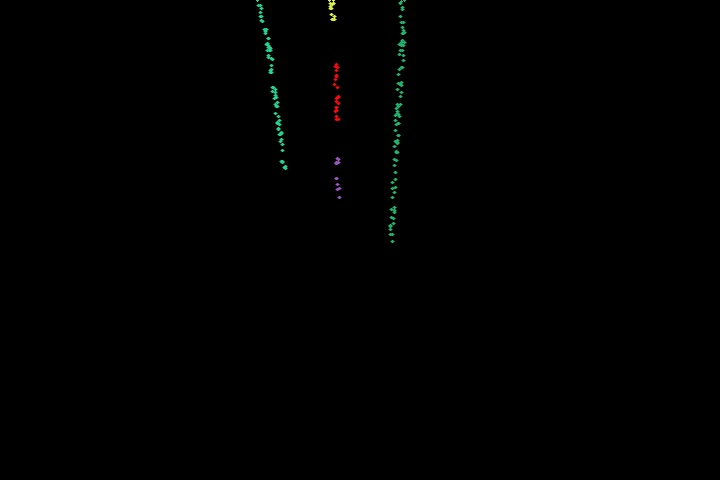
\includegraphics[width=0.5\textwidth]{figures/clusters.jpeg}
    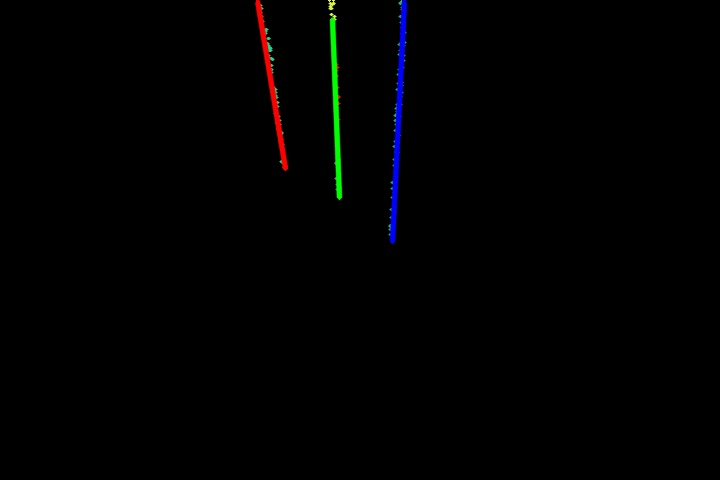
\includegraphics[width=0.5\textwidth]{figures/lines.jpeg}
  }
  \caption{Steps for defining input data for control algorithm. (left:
  clusters, right: 3 lines of input data)}
  \label{fig:inputdata}
\end{figure}
% section Clustering and Pattern Matching (end)

\end{document}
